\chapter{Machine learning challenges}
\label{cha:results}


\section{Natural Language Processing Classification}

When dealing with natural language, one of most important common denominator is how we represent words as input to any of our models. How do we transform sentences/words into numerical vectors.

In this section, we will quickly describe Mikolov's Word2Vec models (Continuous Bag of Word, and Skip-Gram), that proposed a new way to build word embeddings based on words coocurrence in a context window.

Then we will explain in more detail recent work from Facebook, that propose new models based on Mikolov's work, allowing the use of sub-word information, and proposing a novel way to compute classification tasks while learning embeddings.

\subsection{Probability of sequence of tokens}

One solution to extract information from corpus of text is to build a model that will assign a probability to a sequence of tokens. 

Let's consider the following sentence: \say{\textit{To classify you have to learn.}}

A good language model will give this sentence a high probability because this is a completely valid sentence, syntactically and semantically.

Similarly, the sentence \say{Before car bird eating sea.} should have a very low probability because it makes no sense. 

Mathematically, we can call this probability on any given sequence of n words:

\begin{align}
	P(\textit{'To'},\textit{'classify'}, ..., \textit{'learn'})
\end{align}

To make sense, we would like sentences of a given corpus to have a high probability.

Let's introduce the notations for this section:

{\ttfamily
\begin{table}[H]
    \centering
    \begin{tabular}{ll}
        \toprule
        $V$       	   	 &    the ordered vocabulary \\
        $T$    		   	 &    the size of corpus \\
        $w_i$          	 &    the i-th word in corpus \\
        $w_{i^{(v)}}$          	 &    the i-th word in vocabulary \\
        $*i = V(w_{i})$       &    the index of i-th word of corpus in vocabulary V, such as $ w_{i} = w_{*i^{(v)}}$\\
        $C_t^{(c)}$      &    the context of t-th word in corpus, for window of size $c$: $w_{t-c}, ..., w_{t-1}, w_{t+1}, ... ,w_{t+c}$\\
		$\mathbf{x}_i$ 				& one hot word vector corresponding i-th word in vocabulary $V$ \\
        $\mathbf{x}_{(C_t^{(c)})}$ 	& the average of all one hot vectors of words in context $C_t^{(c)}$ \\
        \bottomrule
    \end{tabular}
\end{table}
}

With:
\begin{align}
	v_1 &= 
	\begin{bmatrix} 
		1 \\
		0 \\
		\vdots\\
		0
	\end{bmatrix}
	v_{*1} = 
	\begin{bmatrix} 
		0 \\
		1 \\
		\vdots\\
		0
	\end{bmatrix}
	\textnormal{if } *1 = V(w_1) = 2\\
	\mathbf{x}_{(C_t^{(c)})} &= \frac{\mathbf{x}_{*(t-c)} + \mathbf{x}_{*(t-c+1)} ... + \mathbf{x}_{*(t+c)}}{|C_t^{(c)}|}
\end{align}

Taking our corpus \say{\textit{To classify you have to learn.}}:

\begin{itemize}
	\item our corpus is of size: $T=6$
	\item our vocabulary is: $V =$ (to, classify, you, have, learn), an ordered list of size $|V| = 5$ (word \textbf{to} is present twice in corpus)
	\item $w_5$ is word \textbf{to}, indexed in vocabulary as $*5 = V(w_5) = 1$ (first word of vocabulary)
	\item $\mathbf{x}_{*5} = \begin{bmatrix} 
		1 \\
		0 \\
		\vdots\\
		0
	\end{bmatrix}$
	\item $C_3^{(2)}$ is context of word \textbf{you} with window of size 2: \{to, classify, have, to\}
	\item $x_{(C_3^{(2)})} = 
	(\mathbf{x}_{*1} +\mathbf{x}_{*2} + \mathbf{x}_{*4} + \mathbf{x}_{*5}) / 4 = (\mathbf{x}_{1} +\mathbf{x}_{2} + \mathbf{x}_{4} + \mathbf{x}_{1}) / 4
	=\begin{bmatrix} 
		1/2 \\
		1/4 \\
		0\\
		1/4\\
		0
	\end{bmatrix}$
\end{itemize}


\subsection{Word2Vec models}

Word2vec can utilize either of two model architectures to produce a representation of words: \textbf{continuous bag-of-words} (CBOW) or \textbf{skip-gram}. 

In the continuous bag-of-words architecture, the model predicts the current word from a window of surrounding context words. The order of context words does not influence prediction (bag-of-words assumption). In the continuous skip-gram architecture, the model uses the current word to predict the surrounding window of context words. 
The skip-gram architecture weighs nearby context words more heavily than more distant context words.

Both models can be trained from an unlabeled large corpus of text and rely on the same trick: transform unlabeled data into a labeled dataset for supervised learning to unveil hidden dependencies between words.

Since these two models are quite similar, we will only describe in detail the CBOW in this section.

\subsubsection{CBOW}

In the CBOW model, we try to maximize the likelihood occurence of a word given its context, for a given window size.

Taking our previous corpus: \say{\textit{To classify you have to learn.}}


With a context window of size 2, we can extract many labeled samples:
\begin{itemize}
	\item \textbf{context}: \{classify, you\}, \textbf{target}: to
	\item \textbf{context}: \{to, you, have\}, \textbf{target}: classify
	\item \textbf{context}: \{to, classify, have, to\}, \textbf{target}: you
	\item ...
	\item \textbf{context}: \{have, to\}, \textbf{target}: learn
\end{itemize}


Mathematically, with $w_t$ our target word, $c$ the size of our context window, the probability of our target word given the context can be written as:

\begin{align}
	P(w_t | w_{t-c}, ..., w_{t-1}, w_{t+1}, ... ,w_{t+c}) = P(w_t | C_t^{(c)})
\end{align}

Given a word vocabulary of size $V$, the goal is to learn a vectorial representation for each word $w$. Word representations are trained to \emph{predict well} words that appear in its context.

So given a large training corpus represented as a sequence of words $w_1, ..., w_T$, the objective of the CBOW model is to maximize the following log-likelihood:
\begin{equation*}
  \sum_{t=1}^T \ \log P(w_t \ | \ \mathcal{C}_t^{(c)}),
\end{equation*}

\textbf{Parametrization and model}

The probability of observing a context word $w_t$ given $\mathcal{C}_t^{(c)}$ will be parameterized using the aforementioned word vectors.

We create two matrices $A \in \mathbb{R}^{dim \times |V|}$ and $B \in \mathbb{R}^{|V| \times dim}$, where $dim$ is an arbitrary size which defines the size of our embedding space.

$A$ is the input word matrix such that the *i-th column of $A$ is the dim-dimensional embedded vector for word $w_{i}$ when it is an input to this model. 
Similarly, B is the output word matrix. The *j-th row of B is an dim-dimensional embedded vector for word $w_j$ when it is an output of the model. 



Let's introduce some new notations:

{\ttfamily
\begin{table}[H]
    \centering
    \begin{tabular}{ll}
        \toprule
        $dim$ 				& chosen size for our embeddings \\
        $A$ 				& input word matrix $\in \mathbb{R}^{dim \times |V|}$ \\
        $B$ 				& output word matrix $\in \mathbb{R}^{|V| \times dim}$ \\
        \bottomrule
    \end{tabular}
\end{table}
}

The input matrix A converts our encoded input bag of words ($\mathbf{x}_{(C_t^{(c)})}$) into a representation in a lower dimensionality.

Let's denote our hidden representation:
\begin{align}
 \mathbf{h}_t = A.\mathbf{x}_{(\mathcal{C}_t^{(c)})}
\end{align}

Finally, this hidden representation will be decoded with the output matrix B to be able to compare it with our target word. Since we are in a single labeled multiclass case, the use of softmax function is adapted to sum our probabilities to 1. In short, in CBOW we define the probability of occurence of words each word of the vocabulary, given a context $\mathcal{C}_t^{(c)}$ (our model), as:

\begin{align}
 \mathbf{\hat y}_t = 
	\begin{bmatrix} 
		P(w_{1^{(v)}} | \mathcal{C}_t^{(c)}) \\
		\vdots \\
		P(w_{t^{(v)}} | \mathcal{C}_t^{(c)})\\
		\vdots \\
		P(w_{|V|^{(v)}} | \mathcal{C}_t^{(c)})
	\end{bmatrix} = 
	softmax(B.A.\mathbf{x}_{(\mathcal{C}_t^{(c)})})
\end{align}

Ie $\forall i \in [1, |V|]$:
\begin{align}
 P(w_{i} | \mathcal{C}_t^{(c)})= 
 	&\frac{  [e^{B.A.\mathbf{x}_{(\mathcal{C}_t^{(c)})}}]_i}
 	{\sum_{j=1}^{|V|} [e^{B.A.x_{(\mathcal{C}_j^{(c)})}}]_i} \\
 	\text{      with}& []_i \text{ meaning the i-th element of a vector}
\end{align}


Whereas the true target is noted:
\begin{align}
 \mathbf{y}_t = 
	\begin{bmatrix} 
		0 \\
		\vdots \\
		1 \\
		\vdots \\
		0
	\end{bmatrix} 
	= \mathbf{x}_t
\end{align}


Since $\mathbf{y}_t$ is a one-hot vector, maximizing log-likelihood of $P(w_t | \mathcal{C}_t^{(c)})$ is equivalent to minimizing the cross entropy of $(\mathbf{\hat y}_t, \mathbf{y}_t)$:
\begin{align}
E(\mathbf{\hat y}_t, \mathbf{y}_t) &= - \mathbf{y}_t^{\top} log(\mathbf{\hat y}_t) = - log(P(w_t | \mathcal{C}_t^{(c)}))
\end{align}

We can represent it as the following multilayer network:

\begin{tikzpicture}[shorten >=1pt,->,draw=black!50, node distance=\layersep]
    \tikzstyle{every pin edge}=[<-,shorten <=1pt]
    \tikzstyle{neuron}=[circle,fill=black!25,minimum size=17pt,inner sep=0pt]
    \tikzstyle{input neuron}=[neuron, fill=yellow!50];
    \tikzstyle{output neuron}=[neuron, fill=blue!50];
    \tikzstyle{hidden neuron}=[neuron, fill=red!50];
    \tikzstyle{true neuron}=[neuron, fill=green!50];
    \tikzstyle{annot} = [text width=4em, text centered]

    % Draw the input layer nodes
    \foreach \name / \y / \word in {1/1/to,2/2/classify,3/3/you,4/4/have,5/5/learn}
        \node[input neuron, pin=left: (\textit{\word}) $x_{\y}$ ] (I-\name) at (0,-0.5 -\y) {};

    % Draw the hidden layer nodes
    \foreach \name / \y in {1,...,3}
        \node[hidden neuron] (H-\name) at (\layersep,-1 -\y) {};
    
    % Draw the output layer node

	\foreach \name / \y in {1,...,5}
        \node[output neuron, pin=right:$\hat y_{\y}$ ] (O-\name) at (\layersep*2,-0.5 -\y) {};

    % Draw the true layer node
	\foreach \name / \y / \word in {1/1/to,2/2/classify,3/3/you,4/4/have,5/5/learn}
        \node[true neuron, pin=right:$y_{\y} (\textit{  \word})$ ] (T-\name) at (\layersep*3,-0.5 -\y) {};


    % Connect every node in the input layer with every node in the
    % hidden layer.
    \foreach \source in {1,...,5}
        \foreach \dest in {1,...,3}
            \path (I-\source) edge (H-\dest);

    % Connect every node in the hidden layer with the output layer
    \foreach \source in {1,...,3}
        \foreach \dest in {1,...,5}
	        \path (H-\source) edge (O-\dest);

    % Annotate the layers
    \node[annot,above of=H-1, node distance=2.5cm] (hl) {Hidden layer: $h$ of size \textit{dim}};
    \node[annot,left of=hl] {Input layer: $\mathbf{x}$ (size $|V|$)};
    \node[annot,right of=hl] (ol) {Output layer: $\hat y$ of size $|V|$};
    \node[annot,right of=ol] {Target: $\mathbf{y}$ one hot vector of size $|V|$};

    \node[annot] (A) at (\layersep/2,-5) {$A$};
    \node[annot] (B) at (\layersep*3/2,-5) {$B$};

\end{tikzpicture}

Matrices A and B are updated using gradient descent and gradient retro-propagation. Update formulas can be found in \cite{yolo}

\subsubsection{Using CBOW embeddings for classification}

Using CBOW algorithm would provide you this A matrix, which is basically a lookup table in which you can extract the representation of any word of your vocabulary in your embedding space (of size $dim <<< |V|$).

Word2Vec treats each word in corpus like an atomic entity and generates a vector for each word.

Transforming a text input in a numerical vector is then possible, and your numerical vector could then be used as input for any classification algorigthm to perform classification tasks.

\subsection{Fasttext}

Fasttext, which is essentially an extension of word2vec model, brings two major conceptual changes (in addition to a very efficient C++ implementation):
\begin{itemize}
	\item simulatenous embedding and classification learning: in Word2Vec, we first build our embeddings, and then use it to translate words in features of low dimensionality for further classification. In fasttext, embedding and classification are different layers of a neural network that are trained simultaneously.
	\item use of subword word information, instead of treating only word entities
\end{itemize}

Details can be found in two papers published by Fasttext team: \cite[Enriching Word Vectors with Subword Information]{fasttextEnriching} and \cite[Bag of Tricks for Efficient Text Classification]{fasttextTricks}

\subsubsection{Multiclass classification model}

Let's consider the case where we have a training set of multiclass single-labeled sentences, for instance:
\begin{itemize}
	\item \textbf{feature}: \{I'm hungry\}, \textbf{target}: neutral 
	\item \textbf{feature}: \{Get out\}, \textbf{target}: angry
	\item \textbf{feature}: \{Nice to be there\}, \textbf{target}: happy
	\item ...
	\item \textbf{feature}: \{Do you want this apple\}, \textbf{target}: curious
\end{itemize}
With our target space being: \{happy, angry, neutral, curious\}, of size $K=4$

What fasttext does, is that instead of first learning word embeddings on a corpus of text, it directly uses features to build specialized embeddings for this classification task.

Denoting $\mathcal{Y} = \{y_i\}_{i \in [1, K]}$, and $\mathbf{x}$ the average of one hot-encoded vector of tokens of a feature in vocabulary $V$:
\begin{align}
 \mathbf{\hat y} = 
	\begin{bmatrix} 
		P(y_1 | \mathbf{x}) \\
		\vdots \\
		P(y_i | \mathbf{x})\\
		\vdots \\
		P(y_K | \mathbf{x})
	\end{bmatrix} = 
	softmax(B.A.\mathbf{x})
\end{align}

Ie $\forall i \in [1, K]$:
\begin{align}
 P(y_i | \mathbf{x})= 
 	&\frac{  [e^{B.A.\mathbf{x}}]_i}
 	{\sum_{j=1}^{K} [e^{B.A.x}]_i} \\
 	\text{      with}& []_i \text{ meaning the i-th element of a vector}
\end{align}


Whereas the true target is noted:
\begin{align}
 \mathbf{y} = 
	\begin{bmatrix} 
		y_1 \\
		\vdots \\
		y_i \\
		\vdots \\
		y_K
	\end{bmatrix} 
\end{align}
wich is a one hot encoded vector corresponding to which is this sample label.


The model is very similar to continuous bag of words model, except that instead of using the middle word of CBOW, we directly use a label. The architecture is then:
\begin{tikzpicture}[shorten >=1pt,->,draw=black!50, node distance=\layersep]
    \tikzstyle{every pin edge}=[<-,shorten <=1pt]
    \tikzstyle{neuron}=[circle,fill=black!25,minimum size=17pt,inner sep=0pt]
    \tikzstyle{input neuron}=[neuron, fill=yellow!50];
    \tikzstyle{output neuron}=[neuron, fill=blue!50];
    \tikzstyle{hidden neuron}=[neuron, fill=red!50];
    \tikzstyle{true neuron}=[neuron, fill=green!50];
    \tikzstyle{annot} = [text width=4em, text centered]

    % Draw the input layer nodes
    \foreach \name / \y / \word in {1/1/I,2/2/am,3/3/hungry,4/4/get,5/5/out, 6/6/nice, 7/7/apple}
        \node[input neuron, pin=left:(\textit{\word  }) $x_{\y}$ ] (I-\name) at (0,-\y) {};

    % Draw the hidden layer nodes
    \foreach \name / \y in {1,...,3}
        \node[hidden neuron] (H-\name) at (\layersep,-1 -\y) {};

    % Draw the output layer node
	\foreach \name / \y in {1,...,4}
        \node[output neuron, pin=right:$f_{\y}$ ] (O-\name) at (\layersep*2,-0.5 -\y) {};

    % Draw the true layer node

	\foreach \name / \y / \label in {1/1/happy,2/2/neutral, 3/3/curious,4/4/angry}
        \node[true neuron, pin=right:$y_{\y}$ (\textit{  \label})] (T-\name) at (\layersep*3,-0.5 -\y) {};

    % Connect every node in the input layer with every node in the
    % hidden layer.
    \foreach \source in {1,...,7}
        \foreach \dest in {1,...,3}
            \path (I-\source) edge (H-\dest);

    % Connect every node in the hidden layer with the output layer
    \foreach \source in {1,...,3}
        \foreach \dest in {1,...,4}
	        \path (H-\source) edge (O-\dest);

    % Annotate the layers
    \node[annot,above of=H-1, node distance=2.5cm] (hl) {Hidden layer: $h$ of size \textit{dim}};
    \node[annot,left of=hl] {Input layer: $\mathbf{x}$ (size $|V|$)};
    \node[annot,right of=hl] (ol) {Output layer: $f$ of size $K$};
    \node[annot,right of=ol] {Target: one hot vector $\mathbf{y}$ of size $K$};

    \node[annot] (A) at (\layersep/2,-6) {$A$};
    \node[annot] (B) at (\layersep*3/2,-5) {$B$};

\end{tikzpicture}
Note: 
\begin{itemize}
	\item for readibility just 7 words of the input features are considered.
	\item fasttext first merge all features as one corpus to build vocabulary ($\rightarrow$ size of matrix A)
	\item in practice, dimension of the hidden layer is between 50 and 300
	\item input matrix A embeddings are specialized for this classification task and may not behave well for another classification task
\end{itemize}

\textbf{Subword information}

Each word can be considered as a set of character ngrams. In Fasttext, a word vector is made of the sum of this character n grams. For example the word vector “apple” is a sum of the vectors of the n-grams:
\begin{multicols}{4}
\begin{itemize}
	\item “<ap”, 
	\item “app”, 
	\item ”appl”, 
	\item ”apple”, 
	\item ”apple>”, 
	\item “ppl”, 
	\item “pple”, 
	\item ”pple>”, 
	\item “ple”, 
	\item ”ple>”, 
	\item ”le>”
\end{itemize}
\end{multicols}
Note: this behavious is controlled through hyperparameters controlling smallest ngram size ([minn]) and largest ngram size ([maxn]). For performance and memory size reasons, another hyperparameter ([bucket]) controls the maximum total number of tokens (word tokens + subword tokens).

This provide the following advantages:
\begin{itemize}
	\item Generate better word embeddings for rare words (even if words are rare their character n grams are still shared with other words - hence the embeddings can still be good). In word2vec a rare word (e.g. 10 occurrences) has fewer neighbors to be tugged by, in comparison to a word that occurs 100 times - the latter has more neighbor context words and hence is tugged more often resulting in better word vectors.
	\item Out of vocabulary words - they can construct the vector for a word from its character n grams even if word doesn't appear in training corpus. The choice of hyper parameters controlling the minimum and maximum n-gram sizes has to be chosen.
\end{itemize}

Concretely, the use of subword information will only impact:
\begin{itemize}
	\item how is built the vocabulary. It will not only contain words of the training corpus, but also all ngrams of these words. The vocabulary will thus be much bigger, but with shared properties between different words.
	\item how features are encoded in this vocabulary: 'Do you want this apple' will not be encoded as the average of 5 one hot vectors \{do, you, want, this, apple\}, but as the average of one hot vectors of all tokens contained in the sentence \{<do>, <you, you>, <wa, wan, ant, nt> ...\}.
\end{itemize}

\subsubsection{Miscelanous}

Optimization, hierarchical softmax, negative sampling, word-n-grams, text preprocessing etc..


\subsubsection{Fasttext parameters implementation}

List of all parameters:
\begin{multicols}{3}
\begin{itemize}
	\item \textit{epoch}
	\item \textit{lr}
	\item \textit{lrUpdateRate}
	\item \textit{dim}
	\item \textit{ws}
	\item \textit{loss}
	\item \textit{neg}
	\item \textit{minCountLabel}
	\item \textit{minCount}
	\item \textit{minn}
	\item \textit{maxn}
	\item \textit{bucket}
	\item \textit{t}
\end{itemize}
\end{multicols}

Fasttext implementation lets you choose two parameters to control $\mu$ over time:
\begin{itemize}
	\item \textit{lr}: sets $\mu$ at initialization
	\item \textit{lrUpdateRate}: how continuous \textit{vs} per steps \textit{lr} decays
\end{itemize}

The learning rate $\mu$ decrease linearly, from initial given parameter $lr$ to zero.





\pagebreak
\section{Multilabel classification}

We already studied in previous section how we could compute efficient multi-class classification from natural language input. Yet in our project, most of the product attributes that we wanted to predict were multi-labeled.

In this section, we will first make a quick review of the major algorithms and scoring metrics for multi-label classification, mainly based on the ~\cite[following paper]{MultilabelReview}. Then we will focus on another common approach in neural networks not detailed in the previous paper, that inspired us to modify fasttext algorithm to make it natively support multilabel classification.

\subsection{Review on multi-label classification}

\subsubsection{Scoring metrics}

Multiclass classification metrics in appendix, here only multilabel versions we used.

\subsubsection{Main approaches and algorithms}
\begin{figure}[H]
\centering
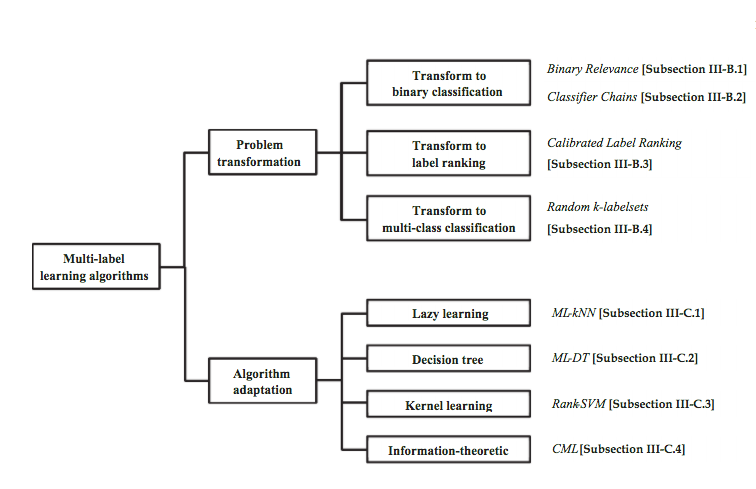
\includegraphics[scale=0.55]{./images/machine-learning/multi-label-approaches.png}
\caption{Categorization of representative multi-label learning algorithms being reviewed, \cite{MultilabelReview}.}
\end{figure}




\subsection{Neural network approach, how we adapted it to Fasttext}

TODO: better introduce.

Suppose a previous layer $h$ (taking a vector x of given size in ouput space of size d) as follow:
\begin{align}
	\mathbf{h}
	&= 
	\begin{bmatrix} 
		h_1 \\
		h_2 \\
		\vdots \\
		h_{\textit{dim}}
	\end{bmatrix}\\ 
	= A^{\top}\mathbf{x}
\end{align}


\begin{align}
	h_j = A^{(j)\top}\mathbf{x}
\end{align}


Let's denote:

\begin{align}
	s_k  = B^{(k)\top} h = \sum_{j=1}^{\textit{dim}} B^{(k)\top}_j h_j 
\end{align}

we can express $f$ as, $\forall k \in [1, K]$:

\begin{align}
	f_k  = \sigma(s_k) = \sigma( \sum_{j=1}^{d} B^{(k)\top}_j h_j) 
\end{align}

Lets consider the following error on one sample $(x, y)$:

\begin{align}
	E = - \sum_{k=1}^K
  			  	\left\{
				    \begin{array}{ll}
				        \log (f_k) & \mbox{if } y_k =1 \\
				        \log (1 - f_k) & \mbox{if } y_k =0
				    \end{array}
				\right.
\end{align}

This error is relevant since the minimization of this error is equivalent to maximizing the maximum of (log-)likelihood.
Plus, it is interpretable: if the $k^{th}$ component $y_k$ is:
\begin{itemize}
	\item positive ($y_k=1$): then the loss increase if $f_k$ is near 0, and decrease if $f_k$ is near 1.
	\item negative ($y_k=0$): then the loss decrease if $f_k$ is near 0, and increase if $f_k$ is near 1.
\end{itemize}



We can represent it as the following multilayer network:


\subsubsection{Gradient retropropagation}


\begin{align}
	\frac{ \partial E } { \partial f_k } = 
		\left\{
		    \begin{array}{ll}
		        - \frac{1}{f_k} & \mbox{if } y_k =1 \\
		        \frac{1}{1 - f_k} & \mbox{if } y_k =0
		    \end{array}
		\right.
\end{align}


\begin{align}
	\frac{ \partial E } { \partial s_k } 
		=  
		\frac{ \partial E } { \partial f_k } \cdot \frac{ \partial f_k } { \partial s_k } 
		&=
		\left\{
		    \begin{array}{ll}
		        - \frac{1}{f_k} \cdot f_k (1 - f_k)& \mbox{if } y_k =1 \\
		        \frac{1}{1 - f_k} \cdot f_k (1 - f_k)& \mbox{if } y_k =0
		    \end{array}
		\right. \\
		&=
		\left\{
		    \begin{array}{ll}
		       f_k - 1 & \mbox{if } y_k =1 \\
		       f_k & \mbox{if } y_k =0
		    \end{array}
		\right. \\
		&= f_k - y_k
\end{align}



\begin{align}
	\frac{\partial E}{\partial B_i^{(k)}} 
	= 
	\frac{\partial E}{\partial s_k} \cdot \frac{\partial s_k}{\partial B_i^{(k)}} 
	= 
	h_i (f_k - y_k)
\end{align}


Trick: derivate $E$ in regard to $s_k$:
\begin{align}
	\frac{\partial E}{\partial h_j} 
	&= 
	\sum_{k=1}^K \frac{\partial E}{\partial s_k} \cdot \frac{\partial s_k}{\partial h_j} \\
	&= 
	\sum_{k=1}^K B_j^{(k)} (f_k - y_k)
\end{align}


\begin{align}
	\frac{\partial E}{\partial A_i^{(j)}} 
	&= 
	\frac{\partial E}{\partial h_j} \cdot \frac{\partial h_j}{\partial A_i^{(j)}} \\
	&= 
	x_i \sum_{k=1}^K B_j^{(k)} (f_k - y_k)
\end{align}


\subsubsection*{Gradient descent}

At each sample $(x, y)$, given a learning rate $\mu$, we update weight as follow:

$B$ weights:
\begin{align}
	B_i^{(k)\mbox{new}} \leftarrow B_i^{(k)\mbox{old}} - \mu (h_i (f_k - y_k))
\end{align}

$A$ weights:
\begin{align}
	A_i^{(j)\mbox{new}} \leftarrow A_i^{(j)\mbox{old}} - 
	\mu 
	\left(
		x_i \sum_{k=1}^K B_j^{(k)\mbox{new}} (f_k - y_k) 
	\right)
\end{align}



\subsection{Multiclass/multilabel scoring metrics}



\pagebreak
\section{Calibration}

After producing our first predictions, we soon realized that we needed more controll on probability scores computed by our models. For some classes, a 0.8 score would on average be right 0.5 of the time, on other classes it could be the opposite, a 0.5 score could be right 0.8 of the time on average.

In this section we will first a naïve calibration implementation, and introduce more commonly adopted strategies.

\subsection{Predictions precision/recall estimation}

\section{Missing labels}

\subsection{Strategies to handle incompletely labeled data}
Consider recall rather than precision. The presence of a lot a FN will impact precision, not recall.

\subsection{Iterative approach to bootstrap new classes}
Manually label some products with new classes, then focus validation on these products. The validated suggestions will be used in next classification workflow.

After some iterations, there might be enough occurences to ensure sufficient scores.

\section{Results}
\subsection{Multiclass}
\subsection{Multilabel}
\subsection{Tuning strategies}

\section{Misc}

\subsection{Dive into kind tree-structure}
\subsection{Enforce better calibration}
\subsection{Tuning strategies}
